\documentclass{beamer}
%[aspectratio=169]   \usepackage[czech]{babel}
\usepackage{apo-lecture}
\usepackage{pdfpages}
\usepackage{pdfcomment}
\usepackage{listings}
\usepackage{array,multirow}

\subtitle{Lekce 07. Vstup a výstup}
\author{Pavel Píša \phantom{xxxxxxxxx} Petr Štěpán \\ \small\texttt{pisa@fel.cvut.cz}\phantom{xxxx}\small\texttt{stepan@fel.cvut.cz}}
\begin{document}

\maketitle

\section{Vstupy a výstupy}

\begin{frame}
\frametitle{Cíl dnešní přednášky}

\begin{itemize}
 \item Projít, jaké jsou možnosti vstupu a výstupu v počítači
 \item Periférie mapované do paměti
 \item Příklady v QtRvSim
 \item PCI a PCIe sběrnice
\end{itemize}
\end{frame}


\begin{frame}[shrink=10]
\frametitle{Architektura počítače -- John von Neumann}
\begin{center}
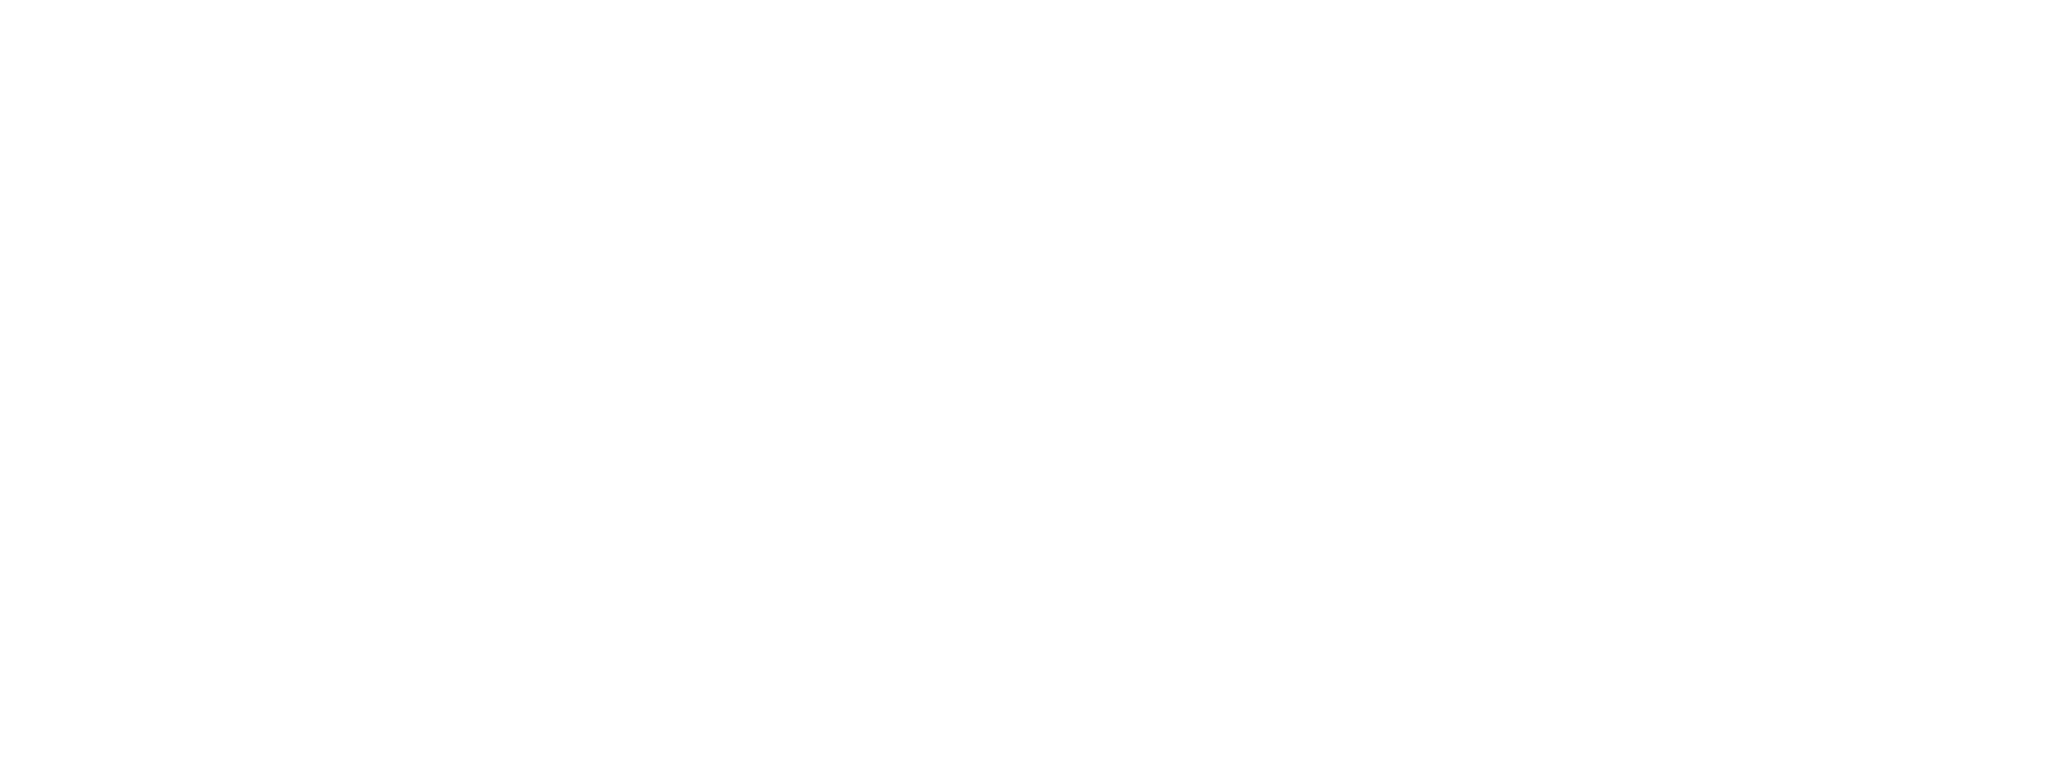
\includegraphics[width=0.5\textwidth]{cpu-vonNeumann.pdf}
\hfill
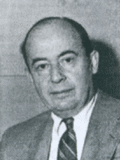
\includegraphics[width=0.15\textwidth]{fig/vonNeumann.png}
\end{center}
\begin{itemize}
\item 5 základních jednotek – řídicí jednotka, aritmeticko-logická jednotka, paměť, vstup (vstupní zařízení), výstup (výstupní zařízení)
\item Architektura počítače by neměla být závislá na řešené úloze, měla by umět provádět program uložený v paměti. Program řídí, co počítač vykonává za instrukce a tím jaké dostane výsledky.
\item Program a data jsou uložena ve stejné paměti, složené z buněk (jednotek) stejné velikosti. Oproti tomu Harvardská architektura měla jeden typ paměti pro program a jiný typ paměti pro data.
\item Další instrukce, která se bude vykonávat je uložena v následující buňce paměti (mimo skoků v programu)
\item Instrukce provádějí aritmetické a logické operace, přesuny dat z/do paměti, skoky a větvení programu a speciální řídicí instrukce.
\end{itemize}
\end{frame}

\begin{frame}
\frametitle{Návrh CPU z přednášky 5}
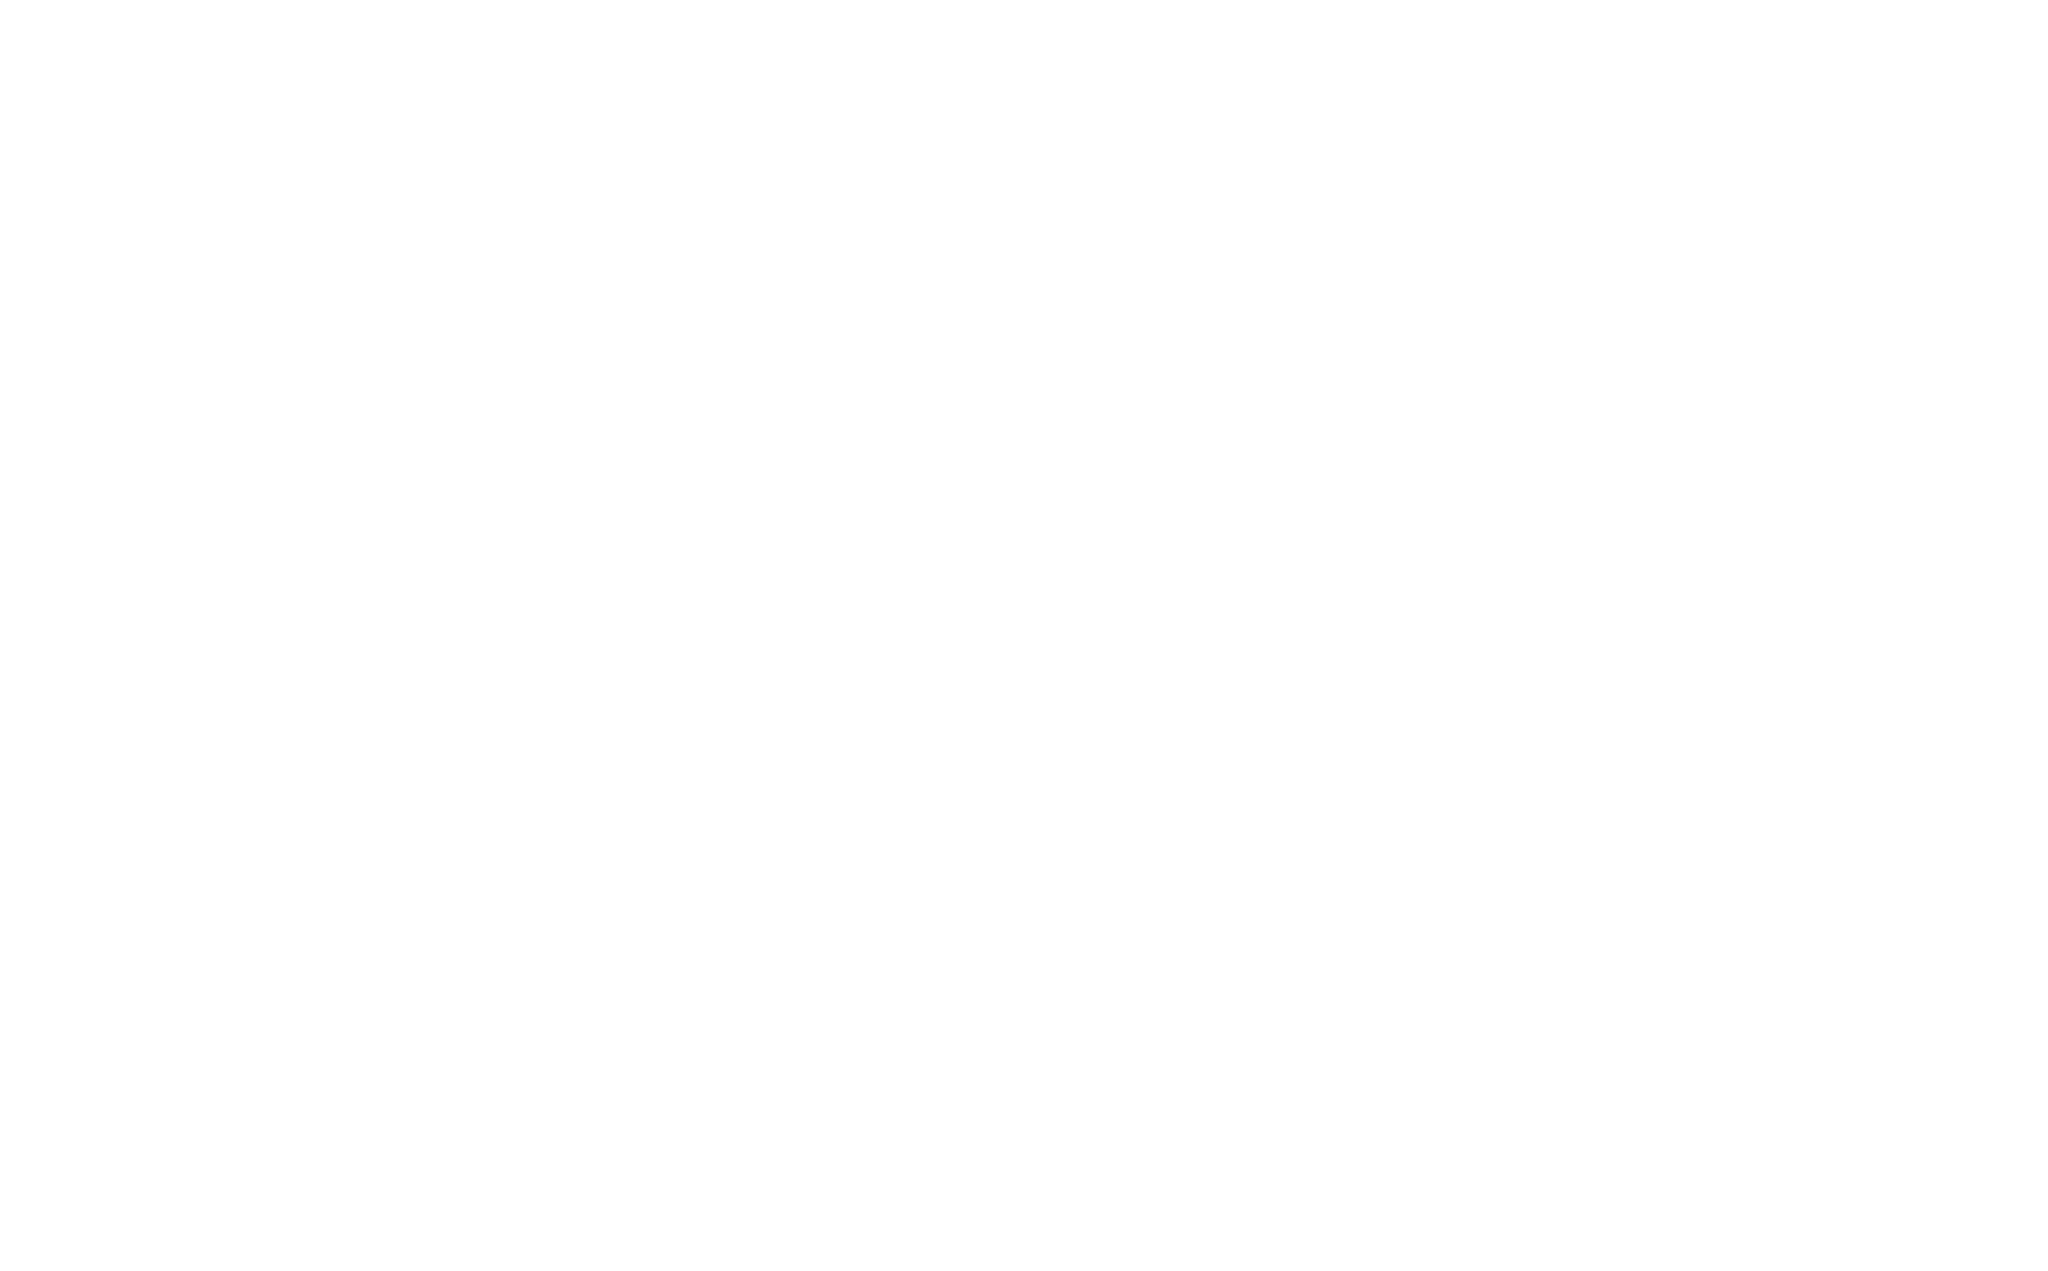
\includegraphics[width=0.95\textwidth]{cpu_design2.pdf}
\end{frame}

\begin{frame}
\frametitle{Propojení CPU s pamětí a perifériemi}
\begin{columns}
\begin{column}{0.4\textwidth}
\end{column}
\begin{column}{0.6\textwidth}  
\begin{itemize}
\item Adresová sběrnice (A0..A31) může být oddělená, nebo multiplexovaná, nebo sdílet stejné signály jako datová část
\item Datová sběrnice (D0..D31) může být obousměrná, nebo oddělená pro každý směr zvlášť, pralelní nebo sériová
\item Řídicí signály sběrnice
\item IOW, IOR se používají pokud jsou vstupní a výstupní periférie oddělené od paměti
\item BE0 to 3 -- pokud je povoleno čtení bajtů na sběrnici širší než 8 bitů.
\end{itemize}
\end{column}
\end{columns}
\end{frame}

\begin{frame}
\frametitle{Klasifikace periférií}
Chování:
\begin{itemize}
\item jenom vstup
\item jenom výstup
\item vstup i výstup (v současnosti většina zařízení)
\end{itemize}

Připojení:
\begin{itemize}
\item přímé propojení CPU a periférie
\item hierarchické -- propojení přes jiné periférie (bridge)
\end{itemize}

Partner:
\begin{itemize}
\item člověk -- jiné parametry komunikace
\item počítač -- většinou rychlejší komunikace
\item prostředí -- senzory a aktuátory
\end{itemize}

Parametry přenosu:
\begin{itemize}
\item kapacita přenosové linky -- maximální možnosti přenosu
\item latence -- čas, do kterého se zareaguje na přenos dat
\end{itemize}
\end{frame}

\begin{frame}
\frametitle{Klasifikace periférií}
Příklady periférií komunikujících s lidmy:
\begin{itemize}
\item klávesnice -- sice jen vstup, ale moderní často i výstup led diody, velmi malá přenosová rychlost, latence až do 200ms 
\item mikrofon/reproduktory -- přenosová rychlost až 8Mbit/s, latence záleží na aplikaci, pro komunikaci
\item tiskárny/scanery -- přenosová rychlost podle připojení, na latency nezáleží (v řádech vteřin)
\end{itemize}

Příklady periférií pro kounikaci mezi počítači
\begin{itemize}
\item modem -- 
\item sítě/WLAN -- 
\item datová úložistě -- HDD, SSD, magnetopáskové jednotky
\end{itemize}

Příklady senzorů a aktuátorů:
\begin{itemize}
\item kamera, laserové hloubkoměry
\item aktuátory -- motory DC/PMSM 
\end{itemize}
\end{frame}

\begin{frame}
\frametitle{Způsoby komunikace s periférií}
Data pouze na dotaz:
\begin{itemize}
\item zařízení čeká, až ho CPU osloví a zašle data na výstup, nebo požádá o připravená data ze vstupu
\item pomalejší komunikace, CPU musí aktivně zjišťovat, zda jsou připravená data k příjmu
\end{itemize}

Periférie využívá přerušení k signalizaci svého stavu:
\begin{itemize}
\item pokud dojde ke změně stavu, periférie vyvolá přerušení (přednáška 9)
\item CPU pak aktivně čte, nebo zapisuje data na periférii
\end{itemize}

Periférie využívá přímý přístup do paměti:
\begin{itemize}
\item často spojeno s vyvoláním přerušení
\item CPU nastaví pouze z/do jaké adresy v paměti se data budou číst/zapisovat a periférie sama řídí přenos dat
\item po ukončení periférie vyvolá přerušení a CPU zkontroluje výsledek přenosu (zda bylo vše v pořádku, nebo došlo k chybě)
\end{itemize}

Programy komunikují s perifériemy pomocí operačního systému a systémového volání a ovladačů periferií(přehled v přednášce 10, podrobně v předmětu OSY).

Další možností je komunikace přes sdílenou paměť -- náplň dnešní přednášky.
\end{frame}



\end{document}

